\chapter{Results: Imaging}
\label{chapter:imaging}

%\emph{\color{red}do corr. on p-meter sensitive A ($\times$1.57) and 89 percent optical flat T}

Results from Ba spectroscopy presented in Chapter \ref{chapter:spectroscopy} were used to determine the best conditions for imaging small numbers of Ba atoms in SXe.  Optimum excitation wavelengths were determined by studying the excitation spectra of the signal as well as the background.  Bleaching studies determined optimum laser intensity to be used.  Deposits made at $50 \pm 5$~K produced more Ba fluorescence signal than those made at 11~K.  Based on these considerations, an image of Ba atoms emitting at 577 and 591~nm is presented in Sec. \ref{sec:imaging590and577} at the level of $\leq 2200$ atoms instantaneously exposed. Images of Ba atoms emitting at 619~nm down to the single-atom level are then presented in Sec. \ref{sec:imaging619}.
%Initial scanned images of Ba\textsuperscript{+} deposits are presented in Sec. \ref{sec:scanning}.



%Aberrations and vibrations in the collection optics could contribute to this, as well as cryostat vibrations.

% inability to reach the diffraction limit in imaging.

%\begin{wrapfigure}{r}{0.5\textwidth}
  %\begin{center}
   % 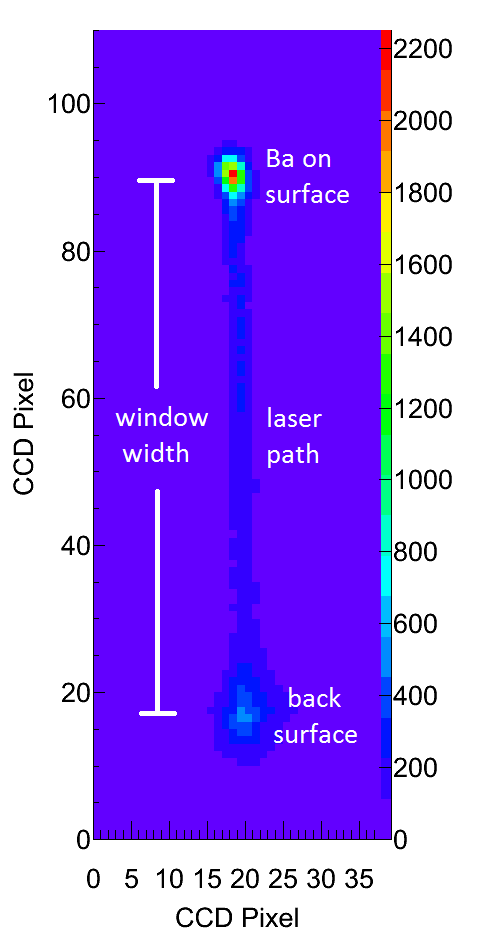
\includegraphics[width=0.35\textwidth]{figures/raw_14-atom_labels_from_paper_1f.png}
  %\end{center}
  %\caption{}
  %\label{fig:imageexamp}
%\end{wrapfigure}

\section{Imaging 577- and 591-nm Fluorescence}
\label{sec:imaging590and577}

\begin{figure} %[H]
        \centering
                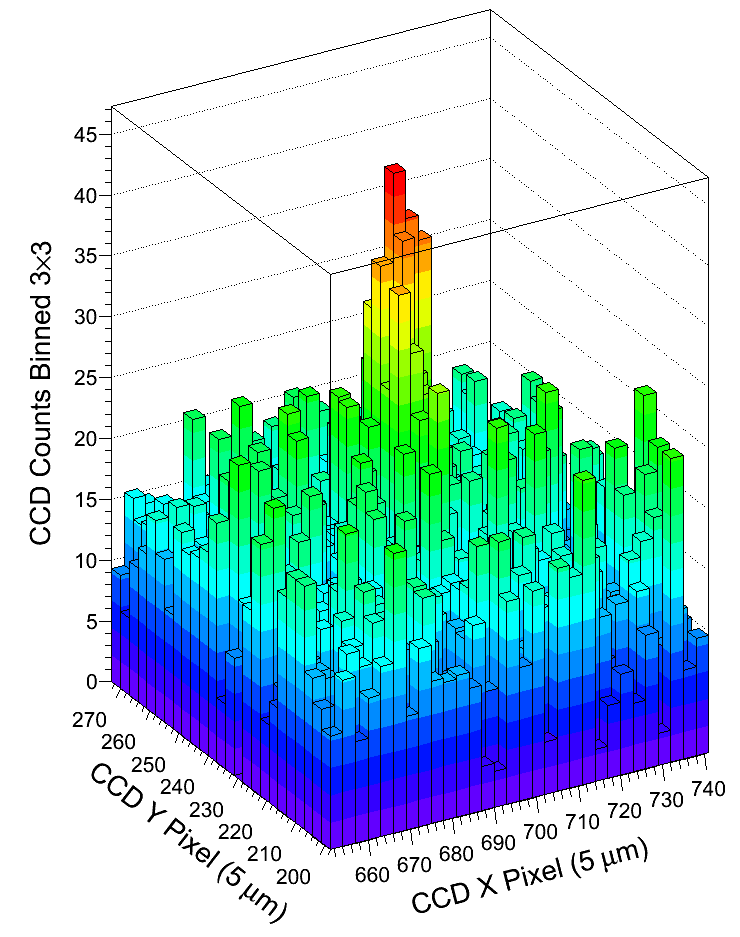
\includegraphics[width=.6\textwidth]{figures/image_1e4.png}
                \caption{Image through 586-nm band-pass filter of $\leq 2200$ Ba atoms in SXe.  The exposure was 100-s with .03~$\mu$W of 566~nm excitation, with a laser beam radius of 5~$\mu$m.  The sample was deposited at 50~K and observed at 11~K.  $3 \times 3$ pixel binning was done with software.}
\label{fig:image590s}
\end{figure}

First attempts at imaging small numbers of Ba atoms in a focused laser region were done with the 577- and 591-nm Ba fluorescence peaks together using a 586-nm band-pass filter, which passes 573 - 599~nm FWHM.  This filter has a 2" diameter, resulting in a nominal collection efficiency of $8.4 \times 10^{-3}$, four times the efficiency given in Table \ref{table:colleff}.  An image of $\leq 2200$ atoms instantaneously in the laser region (see Sec. \ref{subsec:ionDepCal} for calibration of ion deposit) is shown in Fig. \ref{fig:image590s} for a 100-s exposure with 0.03~$\mu$W of 566-nm excitation.  The laser was focused by the bi-convex lens, resulting in a beam radius of 5~$\mu$m, as discussed in Sec. \ref{sec:laser}.  With this spot size, the factor between total and instantaneously exposed atoms is 3, as discussed in Sec. \ref{sec:vibes}, resulting in $\leq 6600$ total atoms exposed.  At this low intensity, little bleaching was observed in the four frames observed (frame 1 is shown).  Groups of 9 ($3 \times 3$) CCD pixels have been binned in software to produce the peak shown.  Detection of single Ba atoms in these sites will require higher laser power to get more photons per atom.  To overcome bleaching at higher intensity, several re-pump lasers will be needed, as discussed in \ref{sec:bleaching}.  As a result of low total exposure, neither the sapphire nor the surface backgrounds are present in these images. 

%$5 \times 10^{3}$        $\leq$ 10$^{4}$

%(10$^{4}$ Ba\textsuperscript{+} ions deposited into the effective laser region)

%Bleaching data was used to optimize laser intensity and exposure time to achieve maximal signal in frame 1, and to avoid hole bleaching.  The fast bleaching of these peaks is the limiting factor on sensitivity.

\begin{figure} %[H]
        \centering
                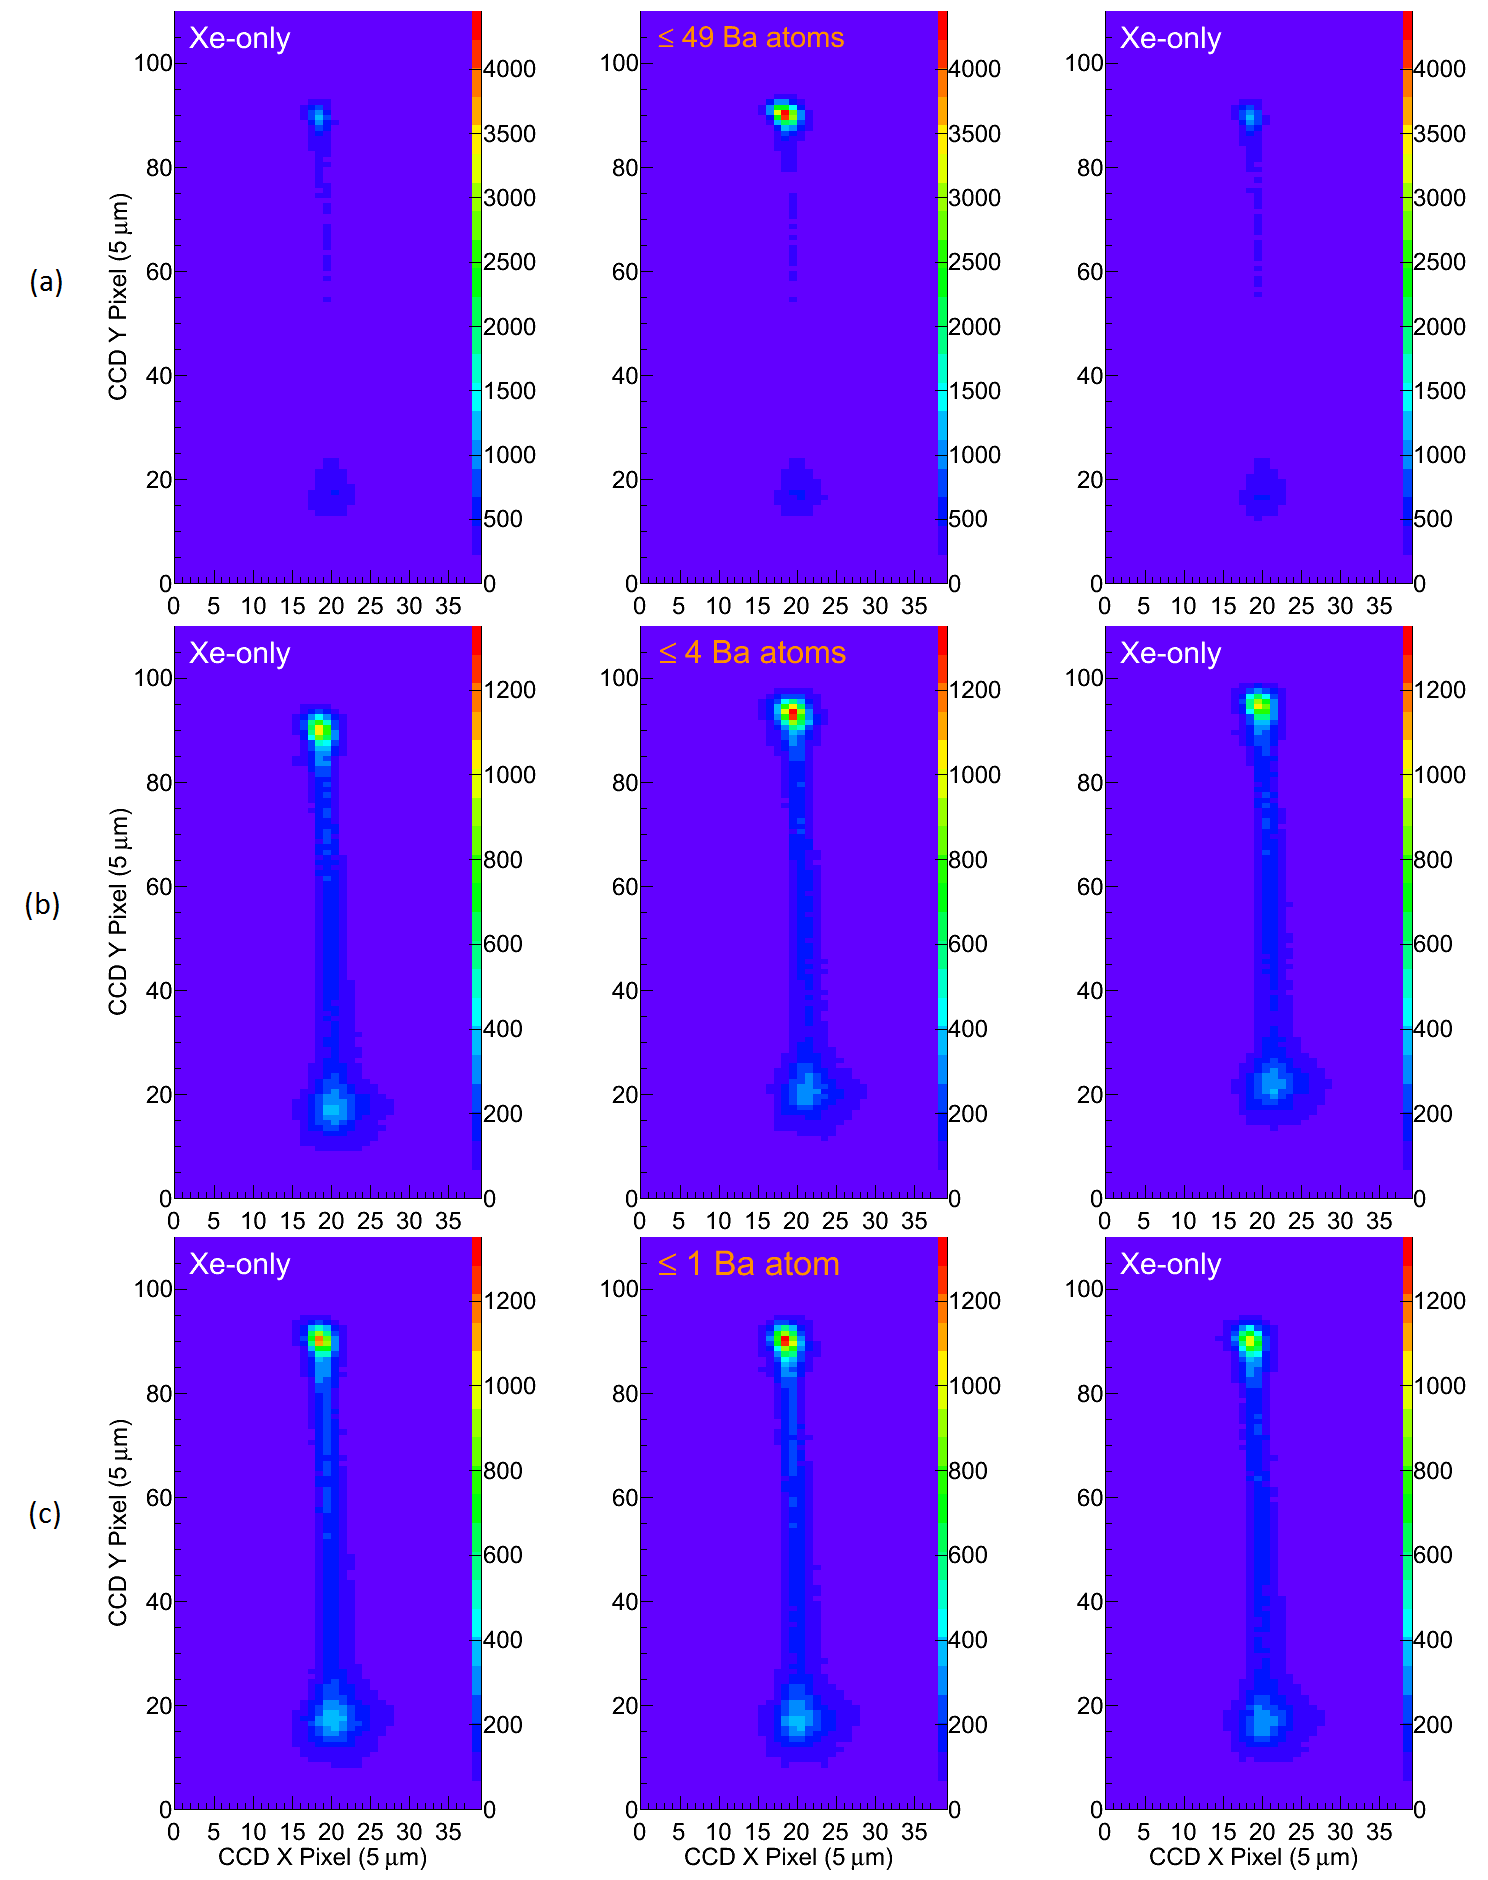
\includegraphics[width=.95\textwidth]{figures/xebaxe_instantaneous_scrunched.png}
                \caption{Raw images through 620-nm band-pass filter of three Ba\textsuperscript{+} deposits yielding (a) $\leq 39$, (b) $\leq 3$, and (c) $\leq 1$ Ba atoms, with their preceding and succeeding Xe-only deposits.  The samples were deposited at 50~K and observed at 11~K.}
\label{fig:xebaxe}
\end{figure}

\section{Imaging 619-nm Fluorescence}
\label{sec:imaging619}

The 619-nm peak has orders of magnitude less bleaching than the 577- and 591-nm peaks.  Thus imaging down to the single atom level is feasible because $10^4$ higher laser intensity can be used.  Raw images of Ba atoms in Ba\textsuperscript{+} deposits and their preceding and succeeding Xe-only deposits are shown in Fig. \ref{fig:xebaxe} for deposits of (a) $\leq 39$ ($\leq 183$), (b) $\leq 3$ ($\leq 14$), and (c) $\leq 1$ ($\leq 5$) instantaneous (total) number of Ba atoms exposed (see Sec. \ref{subsec:ionDepCal} for calibration of ion deposit).  The exposure time is 60~s with around 0.24~mW ($10^4 \times$ that used in Fig. \ref{fig:image590s}) of 570~nm excitation focused to w$_{\text{x}}~\times$~w$_{\text{y}} =$ 2.06~$\mu$m $\times$ 2.66~$\mu$m with the aspherical laser focusing lens and astigmatism compensator (Sec. \ref{sec:laser}).  In this case the factor between total and instantaneously exposed atoms is 4.7 (Sec. \ref{sec:vibes}).  The signal is distinguishable from the background by eye, even with an instantaneous number of exposed atoms at the 1-atom level.

%An imaging experiment consisted of many different pulsed Ba\textsuperscript{+} deposits, each of which was evaporated after observation.  This procedure is described in \ref{sec:deposition}-\ref{sec:collection}.

\begin{figure} %[H]
        \centering
                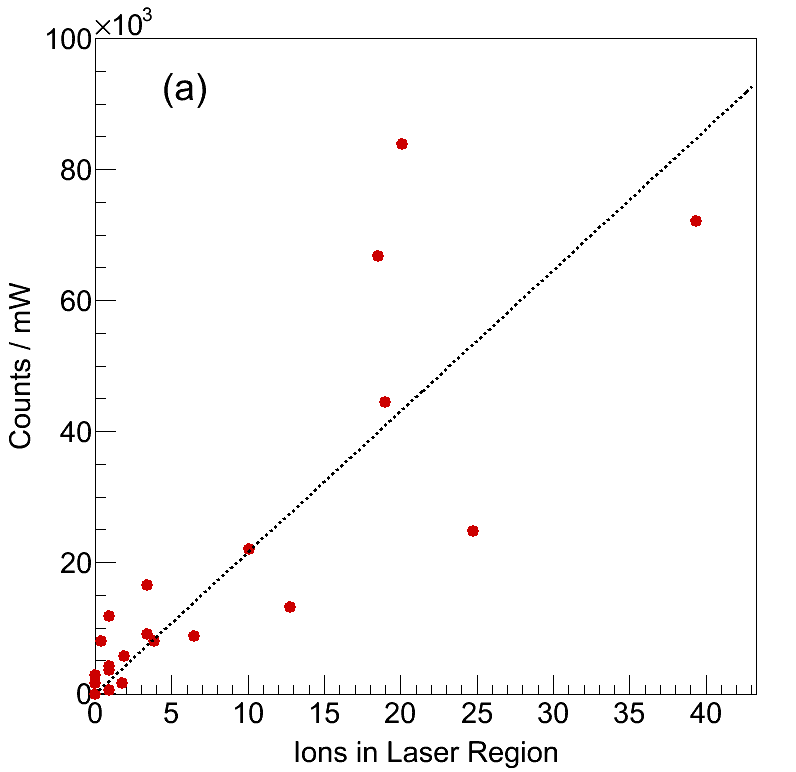
\includegraphics[width=.5\textwidth]{figures/lin_just20150807_lin.png}
                ~
                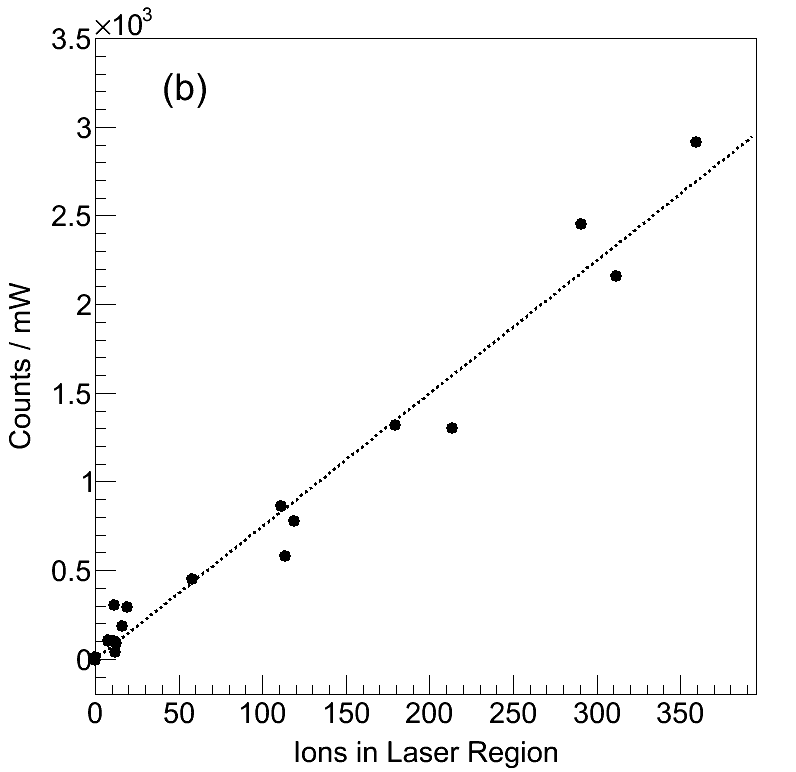
\includegraphics[width=.5\textwidth]{figures/lin_just20150526_lin.png}
                \caption{Total 619-nm signal, scaled by laser power, vs. instantaneous number of Ba\textsuperscript{+} ions deposited inthe focal region of a laser at 570~nm for experiments with (a) aspherical, and (b) bi-convex laser focusing lenses.  The exposure times are (a) 60~s, and (b) 3~s.}
\label{fig:lin}
\end{figure}

\begin{figure} %[H]
        \centering
                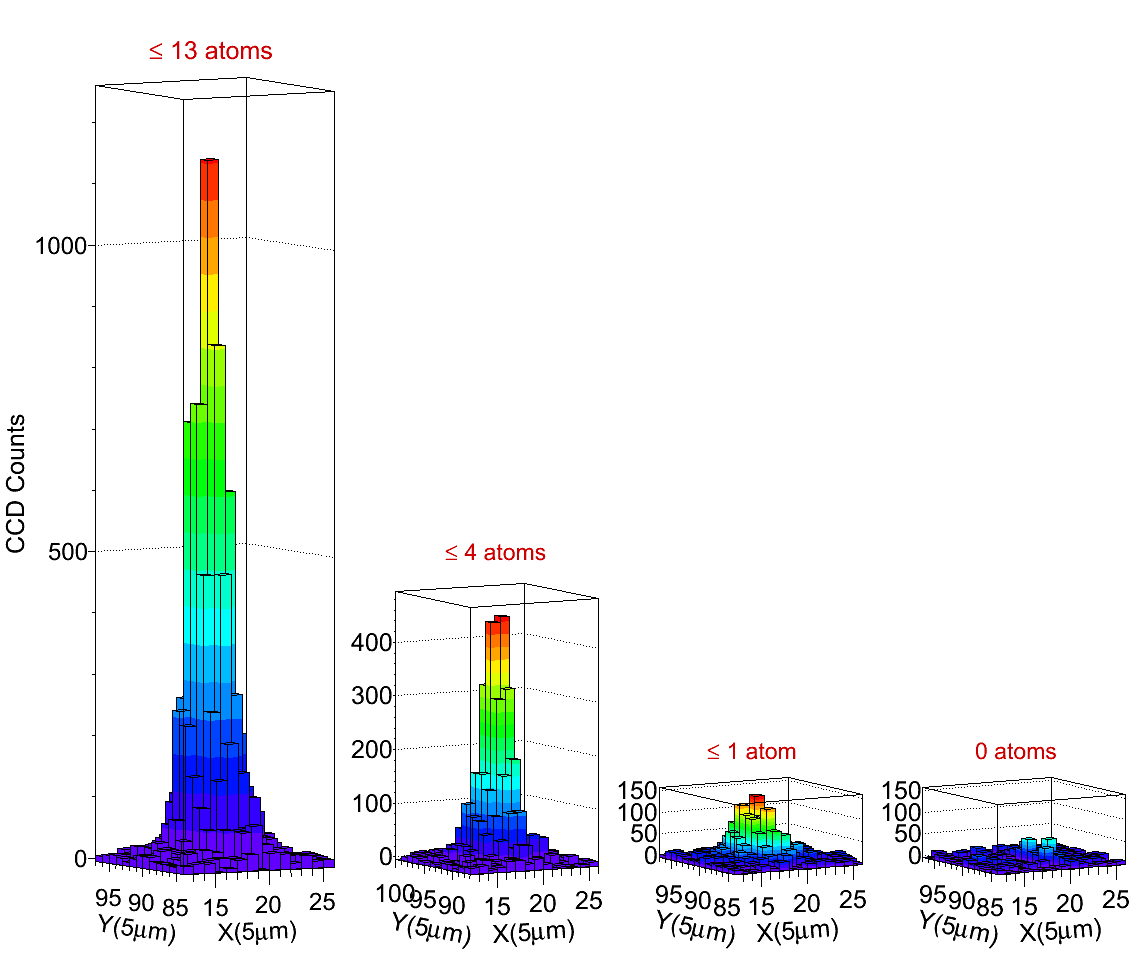
\includegraphics[width=.8\textwidth]{figures/train.png}
                \caption{Subtracted images of 619-nm fluorescence in focused laser region for runs near linear trend line in signal vs. ions deposited.  Exposures are 60~s with around 0.24~mW of 570~nm excitation focused to w$_{\text{x}}~\times$~w$_{\text{y}} =$ 2.06~$\mu$m~$\times$~2.66~$\mu$m.}
\label{fig:train}
\end{figure}

To determine the total 619-nm fluorescence signal level, counts were summed from of a 3-pixel$\times$3-pixel (15$\mu$m$\times$15$\mu$m) region centered on the laser spot in the image.  The background was determined by averaging the 3-pixel$\times$3-pixel sum of the Xe-only runs before and after each Ba\textsuperscript{+} run.  The signal and background were scaled to laser power, and then the background was subtracted.

The integrated 619-nm fluorescence signal is plotted vs. instantaneous number of ions (upper limit on atoms) exposed in Fig. \ref{fig:lin} for many deposits in two experiments with two different laser focusing lenses:  (a) asphere with astigmatism compensation, and (b) bi-convex lens.  The laser and CCD exposures were (a) 60~s with 0.24~mW laser power, and (b) 3~s with 2~mW laser power, respectively.  The two experiments demonstrate a linear relationship between the signal and the number of ions exposed over more than two orders of magnitude.  This is important evidence that the 619-nm peak arises from Ba atoms and not, e.g., Ba$_{2}$ molecules, which would exhibit a quadratic relationship with ions deposited.  Zero-ion deposits are produced by retracting the Faraday cup for 1~s without pulsing the ion beam.  The linear fit in (a), which does not include a constant value, gives a slope of about $2200 \pm 230$~counts/mW per atom with 60-s exposures in a w$_{\text{x}}~\times$~w$_{\text{y}} =$ 2.06~$\mu$m $\times$ 2.66~$\mu$m laser region.  The slope is lower in Fig. \ref{fig:lin}b due to about 5 times larger laser region and 20 times lower exposure time, however signal levels are similar between the two experiments when counts are scaled by time and laser intensity.%Deposits at the single-ion level average to $5000 \pm 2400$~counts/mW.

Images of 619-nm Ba fluorescence are shown in Fig. \ref{fig:train} for a few deposits near the linear trend line in Fig. \ref{fig:lin}a.  In each case the image of the preceding Xe-only deposit is subtracted so that only the Ba fluorescence is seen.  Clear, sharp peaks are observed from an instantaneous number of atoms all the way down to the single-atom level.  This result is a significant advance beyond the sensitivity reported in \cite{Mong2015}, and a major step toward the ultimate success of Ba tagging.  It is generating excitement and interest in the nEXO collaboration.

%, with no clear peak in the zero-atom deposit

\begin{figure} %[H]
        \centering
                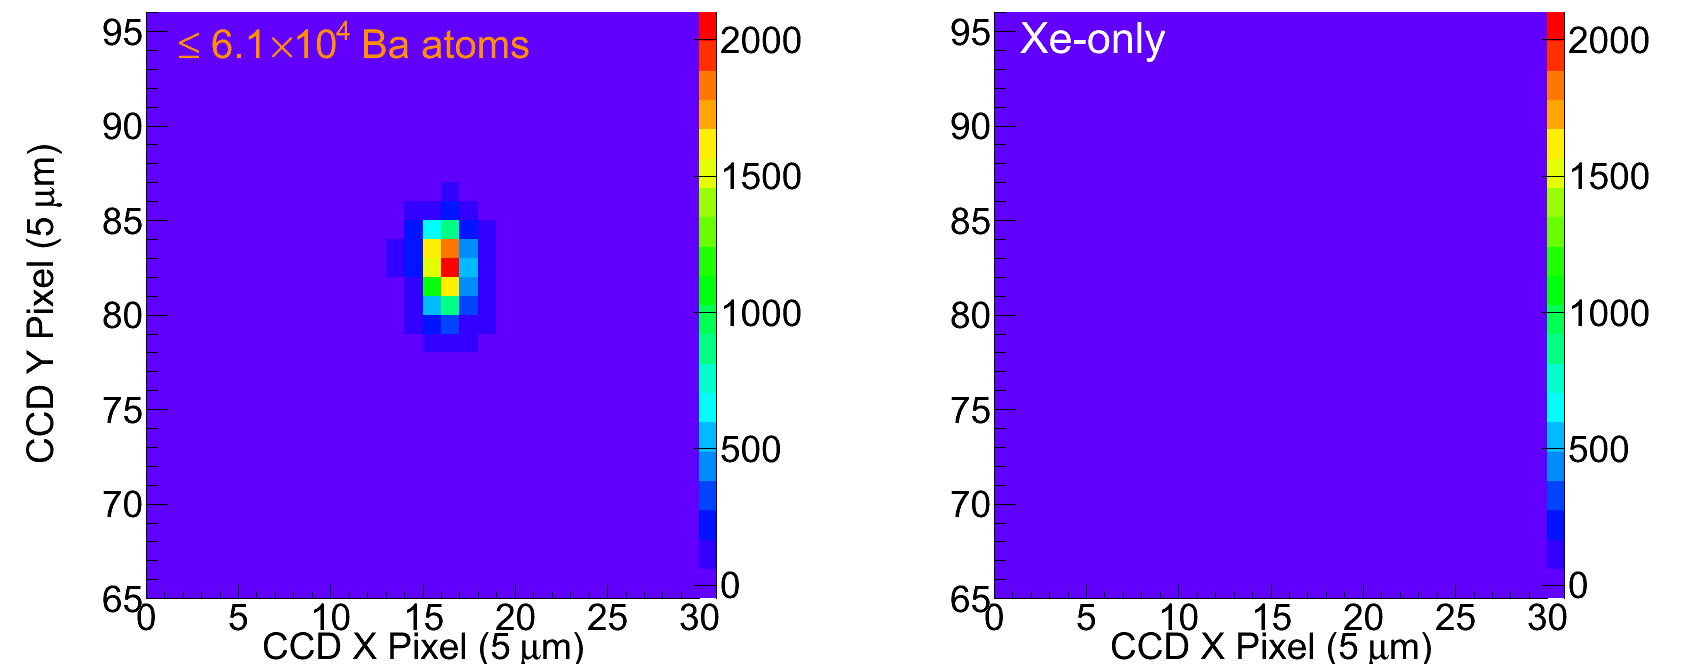
\includegraphics[width=.95\textwidth]{figures/xebaxe_largest_instantaneous.png}
                \caption{Raw images through a 620-nm band-pass filter of a Ba\textsuperscript{+} deposit yielding $\leq 6.1 \times 10^{4}$ Ba atoms, with its succeeding Xe-only deposit.  Exposures are 0.5~s with 0.6~mW of 572~nm excitation focused with the aspherical lens and astigmatism compensator.}
\label{fig:xebaxeLarger}
\end{figure}

Another very significant observation is the lack of Ba fluorescence in Xe-only deposits made after evaporating the matrix, even for large Ba\textsuperscript{+} deposits.  This is demonstrated in Fig. \ref{fig:xebaxe}, where no Ba fluorescence is present in the Xe-only runs following each of the deposits.  This is shown further for a $\leq 61,000$ Ba atom deposit in Fig. \ref{fig:xebaxeLarger}.  The lack of a history effect after evaporation of each sample is important for the implementation of this method of Ba tagging on a probe in nEXO.  Once a Ba daughter has been identified in SXe on a cold probe, the sample can be evaporated without the Ba atom or ion giving false positives in Ba tagging procedures on subsequent $0\nu\beta\beta$ candidate events.

% removed re-pumping section -- double-comment-outs indicate things which were commented out even before this removal

%CORRECTIONS FROM COMMITTEE HAVE NOT BEEN IMPLEMENTED IN THIS SUBSECTION SINCE WE DECIDED TO REMOVE IT
%\section{Scanned Images}
%\label{sec:scanning}

%The ultimate demonstration of single-atom imaging will be to scan the focused laser over samples with more widely separated Ba atoms, observing a peak when the laser moves over individual atoms.  An advantage of scanning is that the resolution in a scanned image is determined by the laser spot size, even when the imaging optics have a lower resolution.  Preliminary scans were performed by scanning the focusing lens in a raster pattern, using the setup described in Sec. \ref{sec:laserscanning}.  Summed counts/mW from a $3 \times 3$ pixel area around the focused laser are plotted vs. raster position for several deposits in Fig. \ref{fig:scans}.  These scans are grids of 20 points in X at about 3.75~$\mu$m/step, by 5 points in Y at about 4.78~$\mu$m/step.  An overall higher signal was observed with 5.7 Ba\textsuperscript{+}/step (d), as well as interesting peak features.  A peak is also observed in the sparse deposit of 0.63 Ba\textsuperscript{+}/step (c).  The aspherical laser focusing lens and astigmatism compensator are used for w$_{\text{x}}~\times$~w$_{\text{y}} =$ 2.06~$\mu$m $\times$ 2.66~$\mu$m 1/e$^{2}$ laser region.  As described in Sec. \ref{sec:vibes}, cryostat vibrations increase the exposed region.  This had the effect of exposing neighboring step regions to the laser, leading to some bleaching during the neighboring step.  Pre-bleaching of the surface background was done with a raster of the dye laser at 580.5~nm, in a $22 \times 7$ grid centered on the $20 \times 5$ grid used during the following experiment, with 10~s at each location.

%\begin{figure} %[H]
%        \centering
%                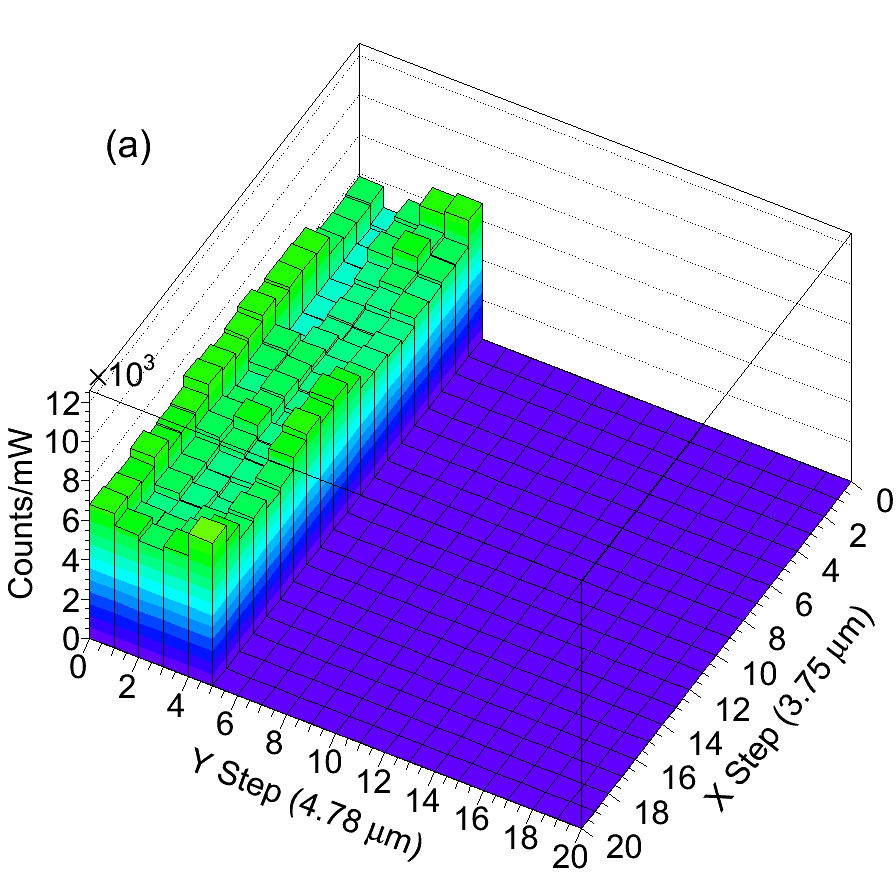
\includegraphics[width=.5\textwidth]{figures/scan_a_0point48Ba_run128.png}
%                ~
%                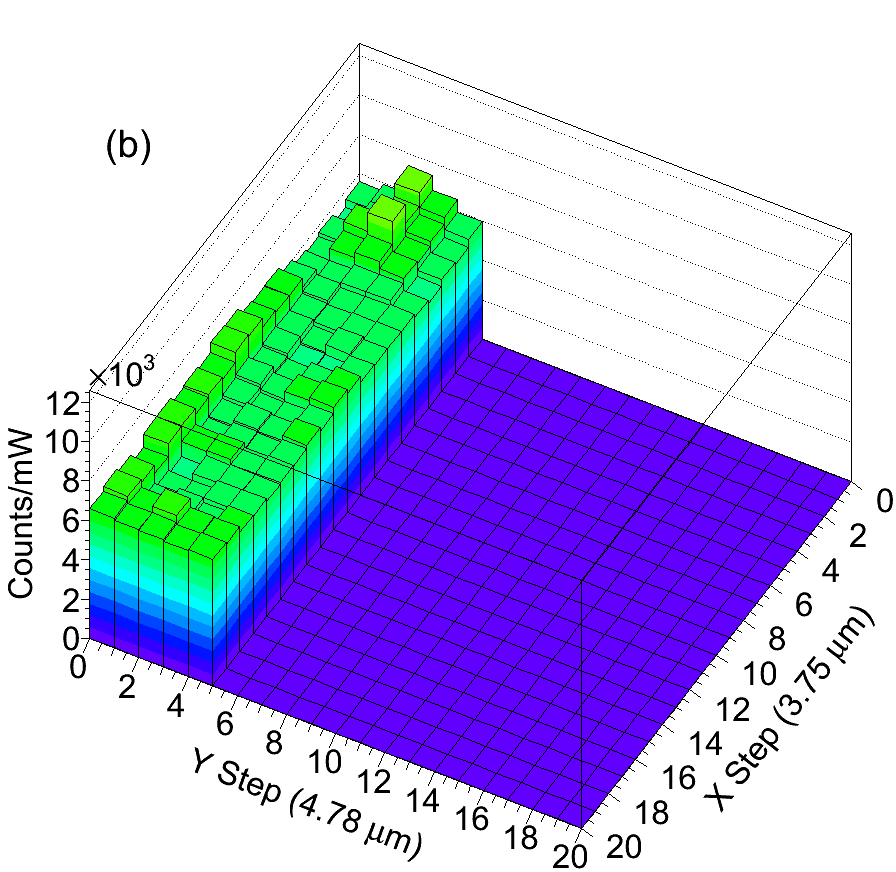
\includegraphics[width=.5\textwidth]{figures/scan_b_Xe_run142.png}
%                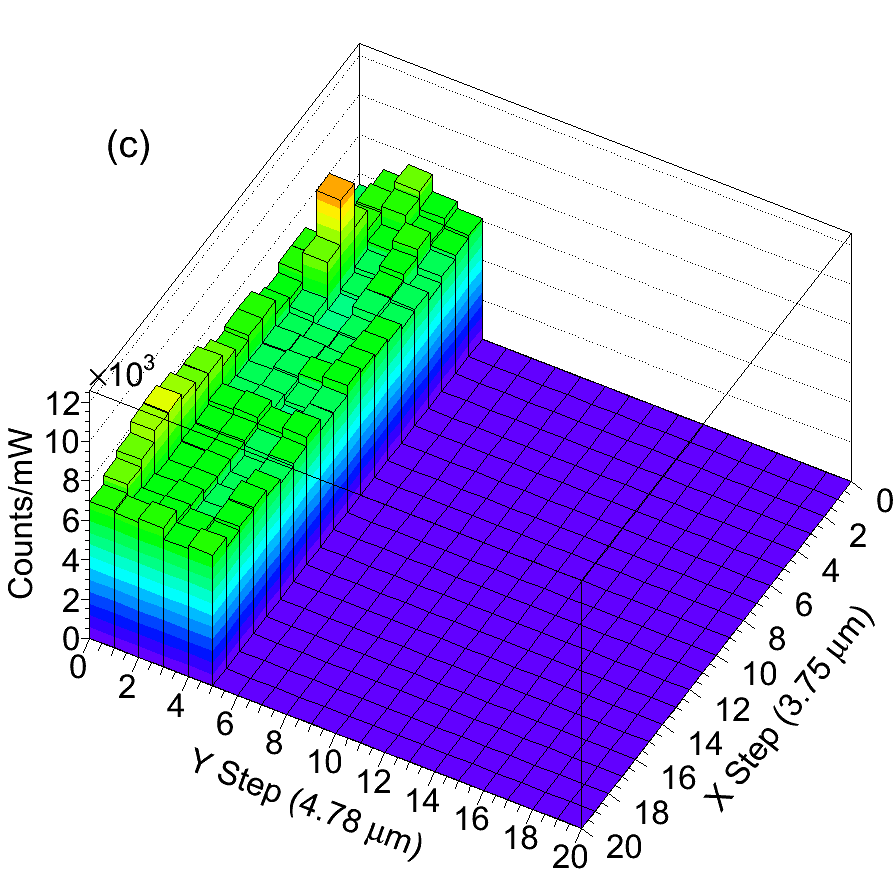
\includegraphics[width=.5\textwidth]{figures/scan_c_0point63Ba_run144.png}
%                ~
%                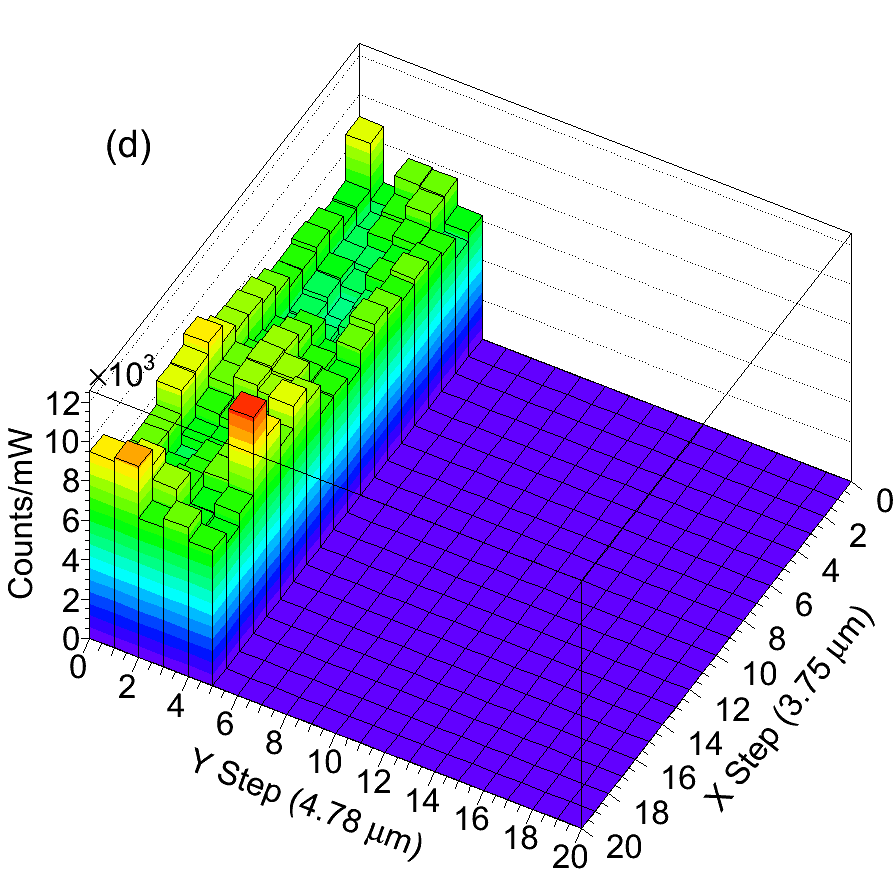
\includegraphics[width=.5\textwidth]{figures/scan_d_5point7Ba_run148.png}
%                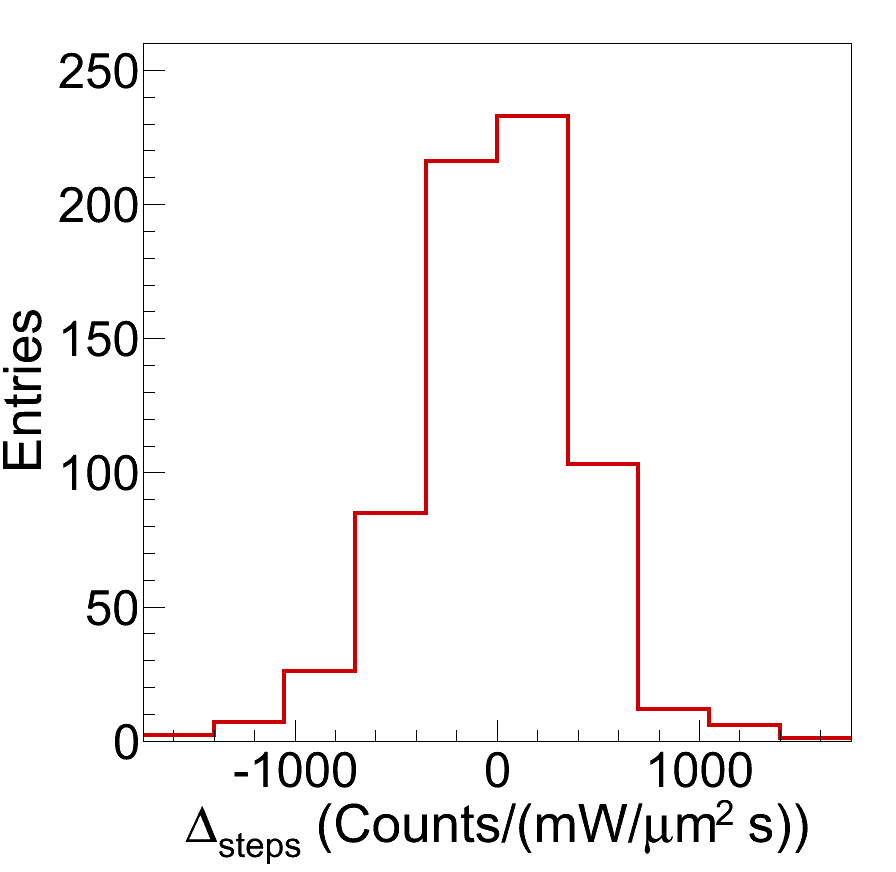
\includegraphics[width=.5\textwidth]{figures/scans_dframeXe.png}
%                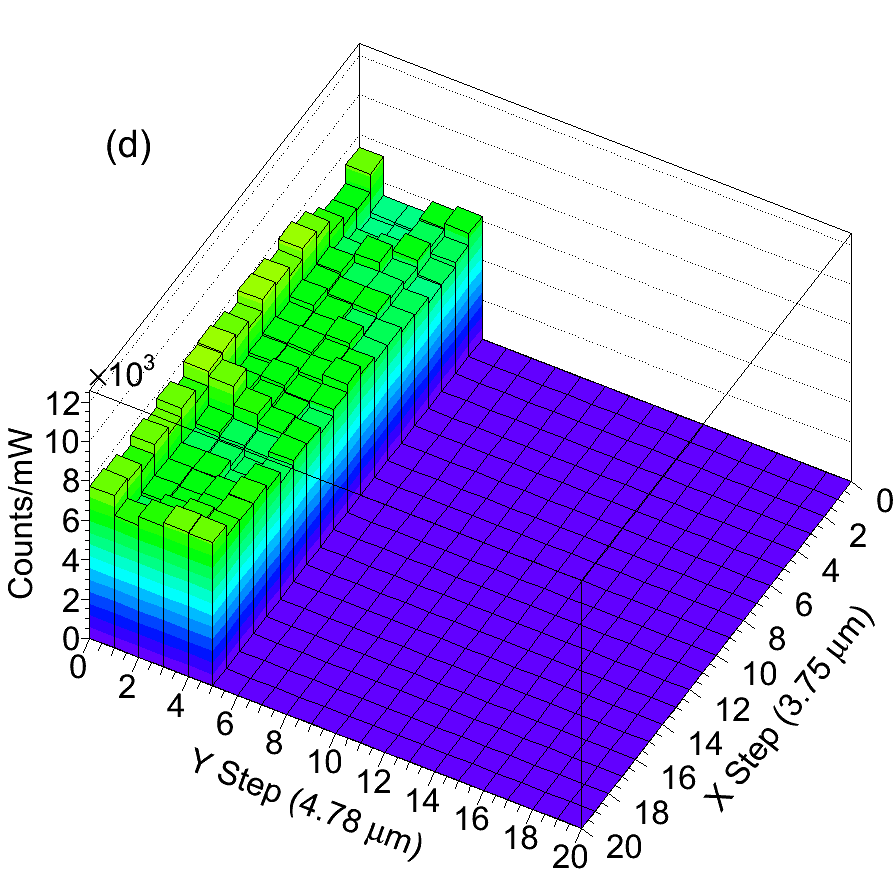
\includegraphics[width=.5\textwidth]{figures/scan_d.png}
%                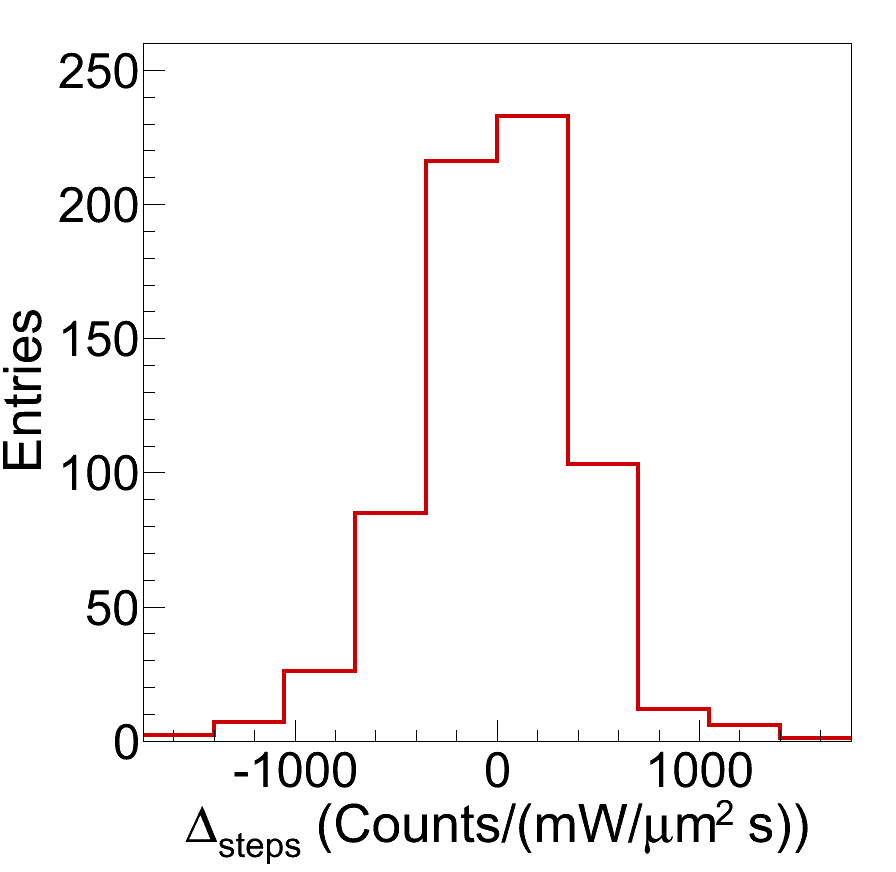
\includegraphics[width=.45\textwidth]{figures/scans_dframeXe.png}
%                \caption{Early attempts at scanned images of a few deposits: (a) 0.48 Ba\textsuperscript{+}/step, (b) Xe-only, (c) 0.63 Ba\textsuperscript{+}/step, and (d) 5.7 Ba\textsuperscript{+}/step.  Exposures are 10-s with 0.4-0.5~mW of focused 570~nm laser.}
%\label{fig:scans}
%\end{figure}
%, and (d) Xe-only

%\begin{figure} %[H]
%        \centering
%                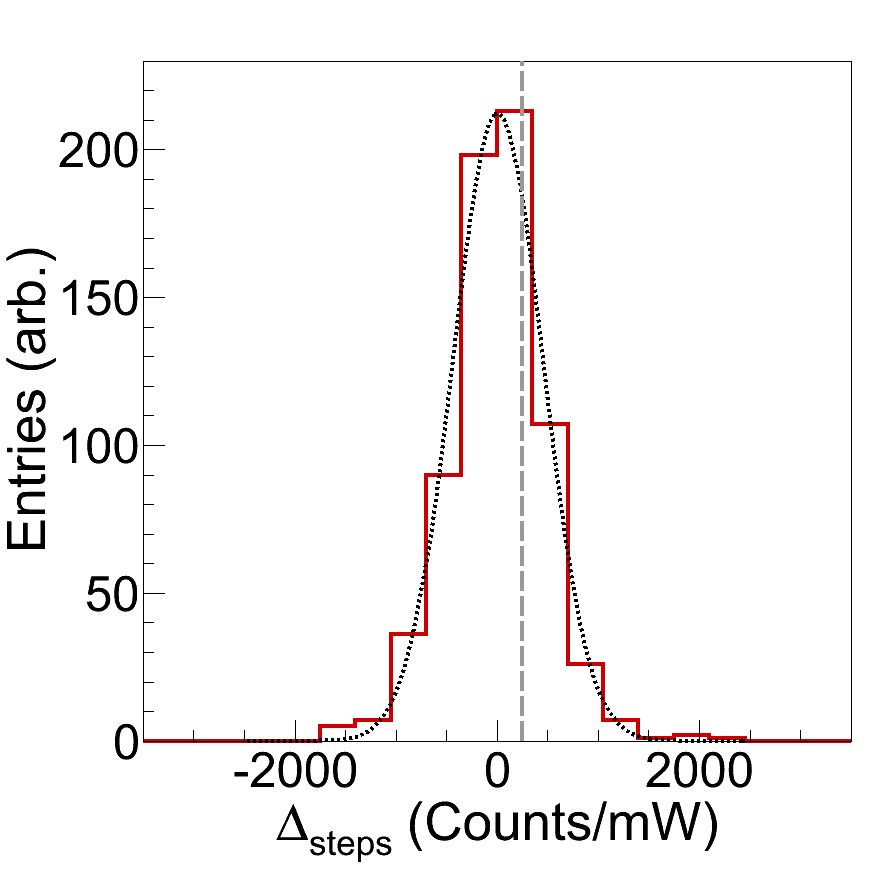
\includegraphics[width=.5\textwidth]{figures/xevarxe_scanDelta_trendline.png}
%                \caption{Distribution of difference in counts ($\Delta_{\text{steps}}$) between successive scan frames in raw Xe-only deposits.}
%\label{fig:scanVarXe}
%\end{figure}

%Signal levels from the scanned images in Fig. \ref{fig:scans} are consistent with previous experiments, with approximately $270 \pm 180$~counts/mW per Ba atom with 10-s exposures.  However, the background level in this particular experiment was somewhat higher, at around 6,000~counts/mW.  The scanned images of Xe-only deposits (Fig. \ref{fig:scans}b) produce a measure of step-to-step variation in the surface background which competes with the single-atom signal.  The difference in counts between successive grid steps is shown as a distribution in Fig.\ref{fig:scanVarXe} for all Xe-only deposits in this set of scanned images.  The single-atom signal level of $250$~counts/mW, acquired from the data set in Figures \ref{fig:xebaxe}, \ref{fig:lin} and \ref{fig:train}, is marked with a gray dotted line.  It is difficult to distinguish single Ba atoms from background fluctuations under these conditions.

%The single-atom signal level of $250 \pm 27$~counts/mW assumes 100\% conversion of deposited Ba\textsuperscript{+} ions.  Thus, it is possible that single Ba atoms produce more signal than this, and that, e.g., the peaks around step (4,1) in Fig. \ref{fig:scans}c and step (16,4) in Fig. \ref{fig:scans}d are due to single atoms.  However, background levels must be reduced further to be sure.  The next steps in scanned imaging of Ba atoms, discussed in Sec. \ref{sec:future}, will involve reducing the surface background.

%\emph{\color{gray}choose what to show and what to say about it -- there are some decent things to show really}  [issues are BG, reproduceability, vibrations]

%\emph{\color{gray}See thought\_process.pptx slide about expected signal / observed BG fluctuation, etc. (unfinished).}